%! Author = wxw85
%! Date = 01/08/2022

\section{Solution}\label{sec:solution}
%**************************************************************
%To solve the problem of visual odometry, we tried different approaches to feed the data into the model, and to construct the model itself.
%We tried following approaches to feed the data:
%\begin{itemize}
%    \item Feeding the sequence into the model directly and presenting the pose as \emph{euler angles}.
%    \item Feeding the sequence into the model directly and presenting the pose as \emph{rotation matrix} so with twelve numbers and \emph{translation vector}.
%    \item Feeding the sequence into the model where the first frame is the origin of the reference frame and presenting the pose as \emph{euler angles}.
%    \item Feeding the sequence into the model where the first frame is the origin of the reference frame and presenting the pose as \emph{rotation matrix} and \emph{translation vector}.
%    \item Feeding the sequence into the model where the first frame is the origin of the reference frame, and using the auto-regressive model to predict the pose.
%\end{itemize}
%
%We used these input strategies to feed the sequence, we tried different variants of models:
%\begin{itemize}
%    \item Using the different version of ResNet (producing \gls{embedding} of size 512 and 2048) model as feature extractor attached to the transformer with only encoder part.
%    \item Using a \gls{mlp} for the images divided into patches to extract the features, and concatenating all the features as a single embedding then feed it into the only-encoder version of transformer.
%    \item Using a MLP for the images divided into patches to extract the features, and concatenating all the features as a single embedding then feed it into the encoder-decoder version of transformer.
%    \item Using the different version of ResNet model as feature extractor attached to the transformer with encoder and decoder.
%    \item The same model as the previous but implemented in \gls{auto-regressive} mode.
%\end{itemize}

We tried to tackle the problem by designing a deep neural network which is composed by a feature extractor, the transformer and a MLP to predict the pose.
We feed the feature extractor with a sequence of images, we tried both grey-scale and RGB images, in this way, we obtain a sequence of embeddings (both size 512 and 2048), the embedding are then fed into the transformer (both encoder and encoder-decoder version) and the output of the transformer is fed into the MLP to predict the pose.

\begin{figure}[H]
    \centering
    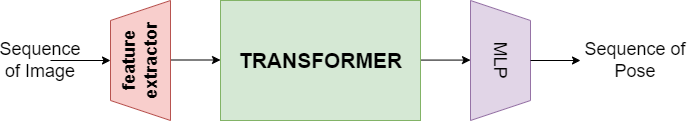
\includegraphics[width=0.8\textwidth]{images/1_4_general_solution}
    \caption{General representation of the model.}
    \label{fig:figure-1_4_solution}
\end{figure}

We use a sequence of image because the transformer model, originally designed for the machine translation, it requires as input a sequence of embeddings, then it outputs another sequence of embeddings.